\documentclass[dvipdfmx]{beamer}
\usepackage{lipsum}
\usetheme{verona}
\usepackage{bxdpx-beamer}
\usepackage{pxjahyper}
\usepackage{minijs}
\usepackage{mathpazo}
\usepackage{amsmath,amssymb}
\usepackage{graphicx}
\usepackage{array}
\usepackage{tikz}
\usepackage{wrapfig}
\usepackage{float}
\usepackage{here}
\usepackage{lscape}
\usepackage{ascmac}
\renewcommand{\kanjifamilydefault}{\gtdefault}
\hypersetup{% hyperrefオプションリスト
 setpagesize=false,
 bookmarksnumbered=true,%
 bookmarksopen=true,%
 colorlinks=true,%
 linkcolor=blue,
 citecolor=blue,
 urlcolor = magenta
}
\setbeamertemplate{navigation symbols}{}

\title[Ang (2021, QJE)]{The Effects of Police Violence on Inner-City Students}
\subtitle{Ang (2021, Quartery Journal of Economics)}
\author[Reviewed by R.TANJI]{Reviewed by Reio TANJI}
\date[Ohtake-Sasaki Seminar]{Jan 13th, 2022 \\ Ohtake-Sasaki Seminar}
\institute[]{Osaka University, Graduate School of Economics}

\begin{document}
\begin{frame}\frametitle{}
\titlepage
\end{frame}

\begin{frame}{Abstract}
  \begin{itemize}
    \item The paper documents racially disparate effects of \textbf{officer-involved killings} occur on the educational and psychological well-being of Los Angeles public high school students.
    \begin{itemize}
      \item In the United States, there occurs nearly 1,000 officer-involved killings.
    \end{itemize}
    \item Exploits hyperlocal variation in how close students live to a killing.
    \item Results: Exposure to police violence leads to
    \begin{itemize}
      \item persistent decreases in GPA
      \item increased incidence of emotional disturbance
      \item lower rates of high school completion and college enrollment.
    \end{itemize}
    \item These effects are driven entirely by black and Hispanic students in response to
    \begin{itemize}
      \item police killings of other minorities
      \item incidents involving unarmed individuals
    \end{itemize}
  \end{itemize}
\end{frame}

\section{Introduction}
\frame{\sectionpage}

\begin{frame}{Literature}
  \begin{itemize}
    \item Police use of force
    \begin{itemize}
      \item are excercised to protect civilians from imminent harm
      \item linked to unfavorable attitudes toward law enforcement.
      \begin{itemize}
        \item Large urban riots in recent U.S. history were all triggered by acts of police violence (DiPasquale and Glaeser, 1998)
        \item Lifetime odds of being killed by police of racial minorities are as high as 1 in 1,000 (Skolnick and Fyfe 1993; Weitzer and Tuch 2004; Brunson and Miller 2005).
      \end{itemize}
    \end{itemize}
    \item Little causal evidence of the social effects on local communities
    \begin{itemize}
      \item Police violence is correlated with homicide and poverty rates (Kania and Mckey 1977; Jacobs, 1998)
      \item Exploiting larger social movement may not be representative (Sigelman et al., 1997; Desmond, Papachristos, and Kirk, 2016; Gershenson and Hayes, 2018).
    \end{itemize}
  \end{itemize}
\end{frame}

\begin{frame}{Dataset and Summary of the Results}
  \begin{itemize}
    \item This paper estimates the short- and long-run effects of police killings on high school students.
    \begin{itemize}
      \item Teenagers face crucial educational decisions
      \item Even vicarious police contact can influence on shaping long-run beliefs and institutional trust (Winfree and Griffith 1977; Leiber, Nalla, and
      Farnworth 1998; Hurst and Frank 2000; Tyler, Fagan, and Geller
      2014)
    \end{itemize}
    \item Novel Datasets
    \begin{itemize}
      \item Incident-level data on the universe
      of officer-involved killings in Los Angeles County (2002-2016)
      \item Individual-level panel data for all high school students enrolled in the Los Angeles Unified School District (LAUSD)
    \end{itemize}
    \item The author calculates each student's geographic proximity to police violence.
    \item Dynamic DID design.
  \end{itemize}
\end{frame}

\begin{frame}{Summary of Results}
  \begin{itemize}
    \item The effects are driven entirely by black and Hispanic students in response to police killings of other underrepresented minorities
    \item Short-run Negative spillovers
    \begin{itemize}
      \item Effects are largest for students who lived closest to the event, and dissipate beyond .50 miles.
      \item GPA: decrease by 0.08 s.d. for several semesters: each hitting affects more than 300 students.
      \item emotional disturbance: 15\% more likely to be classified with PTSD and depression.
    \end{itemize}
    \item Long-run effect: students exposed to officer-involved killings in the 9th grade 
    \begin{itemize}
      \item 3.5\% less likely to graduate from high school.
      \item 2.5\% less likely to enroll college.
    \end{itemize}
    Though smaller in magnitude, effects remain significant in exposure in the 10th and 11th grades.
  \end{itemize}
\end{frame}

\begin{frame}{Contribution}
  \begin{enumerate}
    \item Large externalities of police killings 
    \begin{itemize}
      \item Each officer-involved killing caused three students of color to drop out.
      \item Aggressive policing can socially cost more (Davis, Whyde, and Langton, 2018).
      \item Less extreme uses of force are salient to local residents (Brunson and Miller, 2005; Brunson, 2007; Legewie and Fagan, 2019)
      \item They may be excercised in a racially biased manner (Fryer
      2019).
    \end{itemize}
    \item Self-fulfilling prophecies: minorities believe that police discriminate in use of force (Pew Research Center
    2016, 2019; AP-NORC 2015; Dawson, Brown, and Jackson 2019)
    \begin{itemize}
      \item education (Carlana 2019), labor markets
      (Glover, Pallais, and Pariente 2017), and health care (Alsan and Wanamaker 2018)
      \item Empirical evidence of racial bias is mixed (Nix et al. 2017; Fryer 2019; Johnson et al. 2019; Knox, Lowe, and Mummolo 2020; Knox and Mummolo 2020)
    \end{itemize}
  \end{enumerate}
\end{frame}

\begin{frame}{}
  \begin{enumerate}
    \setcounter{enumi}{2}
    \item Measuring short-run impacts of criminal violence on children (Sharkey, 2010; Sharkey et al., 2012, 2014; Beland and Kim, 2016; Rossin-Slater et al., 2019; Carrell and Hoekstra, 2010; Monteiro and Rocha, 2017; Gershenson and Tekin, 2018)
    \begin{itemize}
      \item Unlike others forms of violence, violence to enforce laws improves public outcomes.
      \item The findings will serve important inputs for pressing policy discussions around police oversight and officer use of force.
    \end{itemize}
    \item Link between neighborhoods and economic mobility (Katz, Kling, and Liebman 2001; Chetty, Hendren, and Katz 2016)
    \begin{itemize}
      \item Intergenerational mobility differs dramatically between blacks and whites: Chetty et al. (2020)
      \item Results suggest that law enforcement may
      play an important role in explaining this racial disparity
    \end{itemize}
  \end{enumerate}
\end{frame}

\section{Background and Data}
\frame{\sectionpage}

\begin{frame}{Los Anageles, California}
  \begin{itemize}
    \item A natural setting for the research.
    \item Today, Los Angeles experiences more police killings than any other county in the nation.
    \begin{itemize}
      \item From Jjuly 2002 to June 2016, 627 officer-involved fatalities occurred (twice as that in New York or Chicago)
    \end{itemize}
    \item two of the most high-profile acts of police violence in U.S. history
    \begin{itemize}
      \item 1965, a 21-year-old African American: 34 deaths and more than 3,000 arrests 
      \item 1992, a 26-year-old black man:  63 deaths, more than 12,000 arrests, and \$1 billion damage in properties.
    \end{itemize}
  \end{itemize}
\end{frame}

\begin{frame}{Police Killings}
  \begin{itemize}
    \item Unique incident-level data on police killings
    \begin{itemize}
      \item From the \textit{Los Angeles Times} Homicide Database
      \item records the followings of all deaths in the county by a "human hand".
      \begin{itemize}
        \item about the deceased: name, age, and race
        \item about the event: exact address and date
      \end{itemize}
      \item contextual details are supplemented by Los Angeles County district attorney incident reports and other sources.
      \begin{itemize}
        \item investigative evidence and officer and witness testimonies
        \item legal analysis of officer actions.
      \end{itemize}
      \item Contextual information for 556 killings.
      \begin{itemize}
        \item whether a weapon was recovered from the deceased
        \item if so, what type (Knife, Gun)
        \item whether the deceased had fired his weapon
      \end{itemize}
    \end{itemize}
    \item In many cases, police actions were predicated on faulty or misreported information
  \end{itemize}
\end{frame}

\begin{frame}{Student Data}
  \begin{itemize}
    \item LAUSD administrative data
    \begin{itemize}
      \item Individual-level records for all high school students in the district from the 2002-2003 to 2015-2016 academic years
      \item 712,954 unique students (anonymized).
      \item demographic information:
      \begin{itemize}
        \item race 
        \item date of birth 
        \item parental education 
        \item home language 
        \item free/subsidized lunch status
        \item proficiency on eighth-grade standardized tests
      \end{itemize}
      \item Each student's last reported home address while enrolled at LAUSD
    \end{itemize}
  \end{itemize}
\end{frame}

\begin{frame}{}
  \begin{itemize}
    \item Measures of academic achievement: observed for grades 9th through 12th
    \begin{itemize}
      \item Semester GPA: average grades in math, science, English, and social sciences
      \item Daily attendance ('09-'10 and onward)
      \item high school graduation: high school diploma or equivalent (GED or CHSPE) or a Special Education Certificate of Completion
      \item college enrollment: whether students enrolled in postsecondary schooling for those who graduated from LAUSD between 2009 and 2014
    \end{itemize}
    \item Mental health
    \begin{itemize}
      \item "emotionally disturbed": certified learning disability that "cannot be explained by intellectual, sensory or health factors" (2004 school year onward)
      \item School Experience Survey (SES): 2014-2015 and 2015-2016 academic years.
      \begin{itemize}
        \item three questions examining feelings of school and neighborhood safety.
      \end{itemize}
    \end{itemize}
  \end{itemize}
\end{frame}

\begin{frame}{}
  \begin{figure}
    \centering
    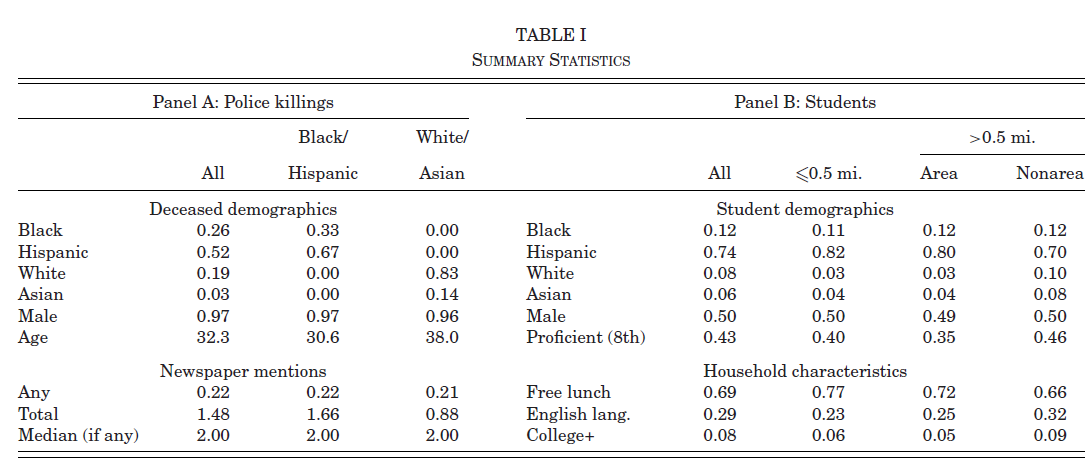
\includegraphics[scale = .45]{fig_tab/os20220113/T1}
    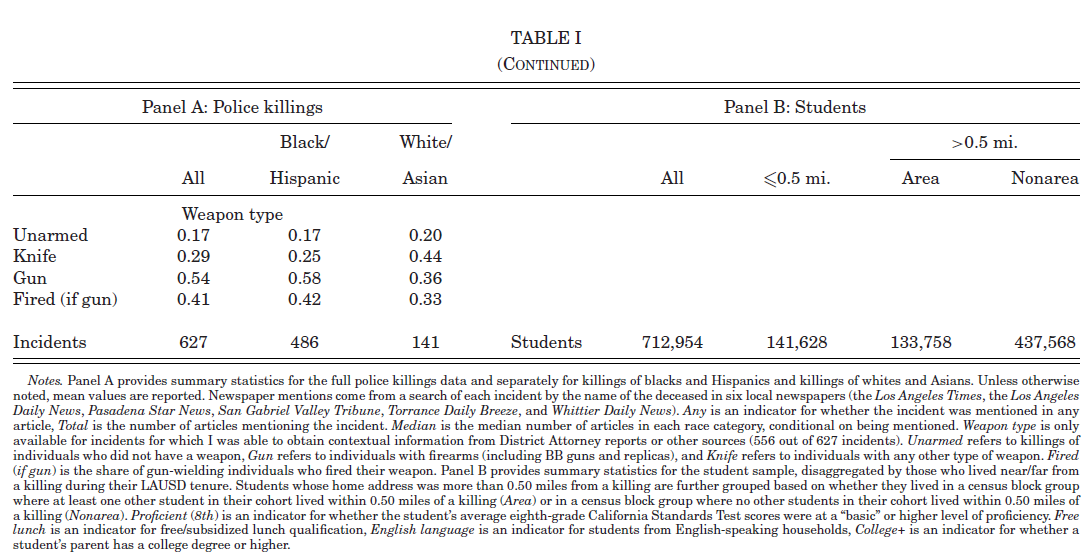
\includegraphics[scale = .45]{fig_tab/os20220113/T1_1}
  \end{figure}
\end{frame}

\begin{frame}{}
  \begin{figure}
    \centering
    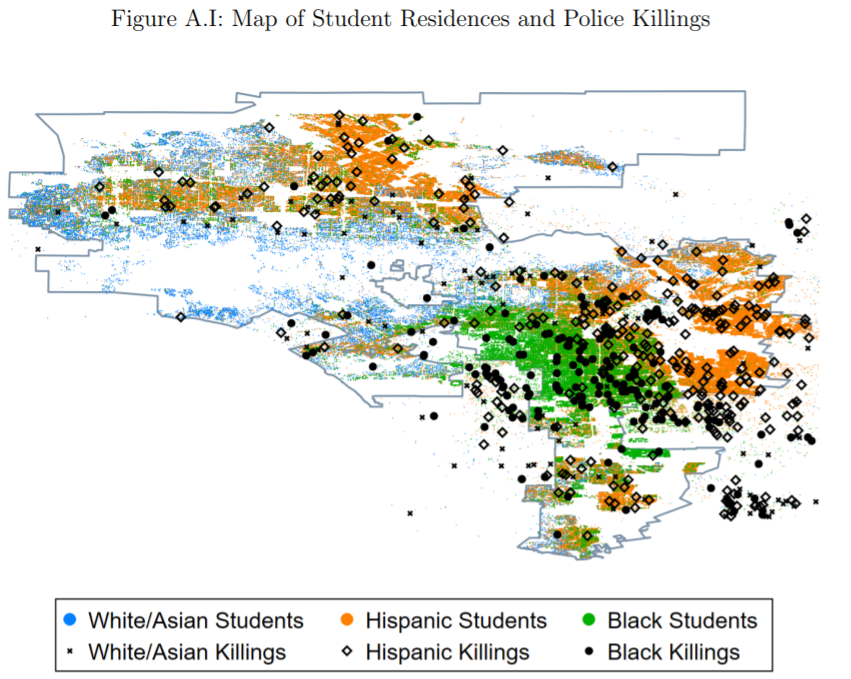
\includegraphics[scale = .55]{fig_tab/os20220113/FA1}
  \end{figure}
\end{frame}

\section{Identification Strategy}
\frame{\sectionpage}

\begin{frame}{Exposure to Police Killings}
  \begin{itemize}
    \item The primary obstacle to identification: correlation with neighborhood characteristics.
    \begin{itemize}
      \item police killings may be more likely to occur where poverty and crime are.
    \end{itemize}
    \item To deal with this problem, the author exploit hyperlocal variation in exposure to killings.
    \begin{itemize}
      \item comparing changes over time among students who lived very close (.50 miles) to a police killing to students who lived slightly farther away
      \begin{itemize}
        \item Killings are quite rare and difficult to predict.
        \item Underreported nature of officer-invoked killings (20\% of media coverage)
      \end{itemize}
    \end{itemize}
    \item Grahpical evidence shows that incidents affect absenteeism of only the students (Chetty et al. 2018, 28).
  \end{itemize}
\end{frame}

\begin{frame}{}
  \begin{figure}
    \centering
    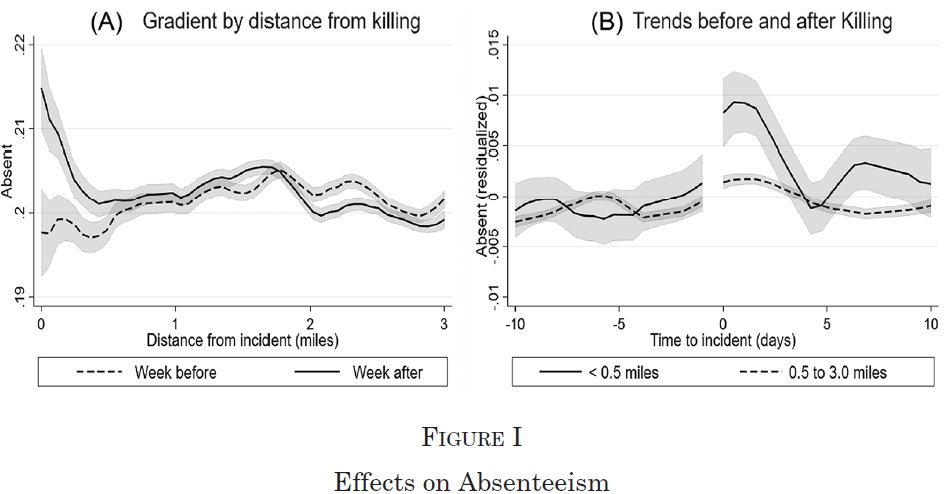
\includegraphics[scale = .6]{fig_tab/os20220113/F1}
  \end{figure}
  \begin{itemize}
    \item the full sample includes more than 600 incidents spread across 15 years and thousands of square miles
  \end{itemize}
\end{frame}

\begin{frame}{Estimating Equation}
  \begin{itemize}
    \item Semester GPA: for individual $i$ at semester $t$ (cohort $c$, neiborhood $n$),
    \[y_{i, t} = \delta_i + \lambda_{n, t} + \omega_{c, t} + \sum_{\tau = -7}^7 \beta_{\tau} \textit{Shoot}_{\tau} + \epsilon_{i, t}\]
    \begin{itemize}
      \item $\delta_i, \lambda_{n, t}, \omega_{c, t}$: individual, neighborhood-semester, and cohort-year fixed effects, respectively.
      \item ${Shoot}_{\tau}$: relative time to treatment. Baseline: $\tau = -1$.
      \item Treatment is defined by the earliest nearby killing if he or she faced multiple ones during high school.
    \end{itemize}
    \item Treatment 
    \begin{itemize}
      \item On average, this captures 303 students per incident.
      \item Roughly 20\% of the sample is ever-treated based on this
      definition.
    \end{itemize}
  \end{itemize}
\end{frame}

\section{Main Results}
\frame{\sectionpage}

\begin{frame}{Academic Performance}
  \begin{figure}
    \centering
    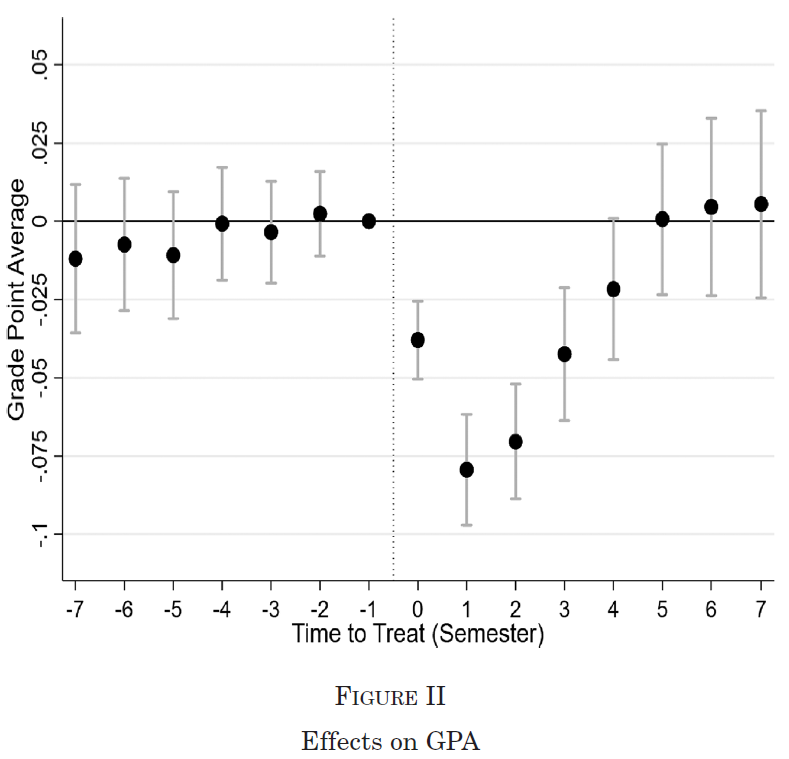
\includegraphics[scale = .55]{fig_tab/os20220113/F2}
  \end{figure}
\end{frame}

\begin{frame}{}
  \begin{itemize}
    \item Prior to shootings, I find little evidence of differential group trends.
    \begin{itemize}
      \item Pretreatment estimates are also jointly insignificant $(F = 0.69, p = .655)$.
    \end{itemize}
    \item GPA declines by 0.04 points in the semester of the shooting and by between 0.07 and 0.08 points in the following two semesters (GPA mean = 2.08, std. dev. = 1)
    \begin{itemize}
      \item Effects then gradually dissipate (reach insignificance five semesters after exposure).
    \end{itemize}
    \item the mean posttreatment estimate of -0.030 std. dev.
    \begin{itemize}
      \item larger in absolute magnitude than the average impact of randomized interventions (Fryer 2017)
      \begin{itemize}
        \item providing student incentives: -0.024 s.d.
        \item low-dosage tutoring: 0.015 s.d.
        \item choice and vouchers: 0.024 s.d.
      \end{itemize}
      \item 1.3 percentage point decrease in the graduation rate
    \end{itemize}
  \end{itemize}
\end{frame}

\begin{frame}{Psychological Well-Being}
  \begin{figure}
    \centering
    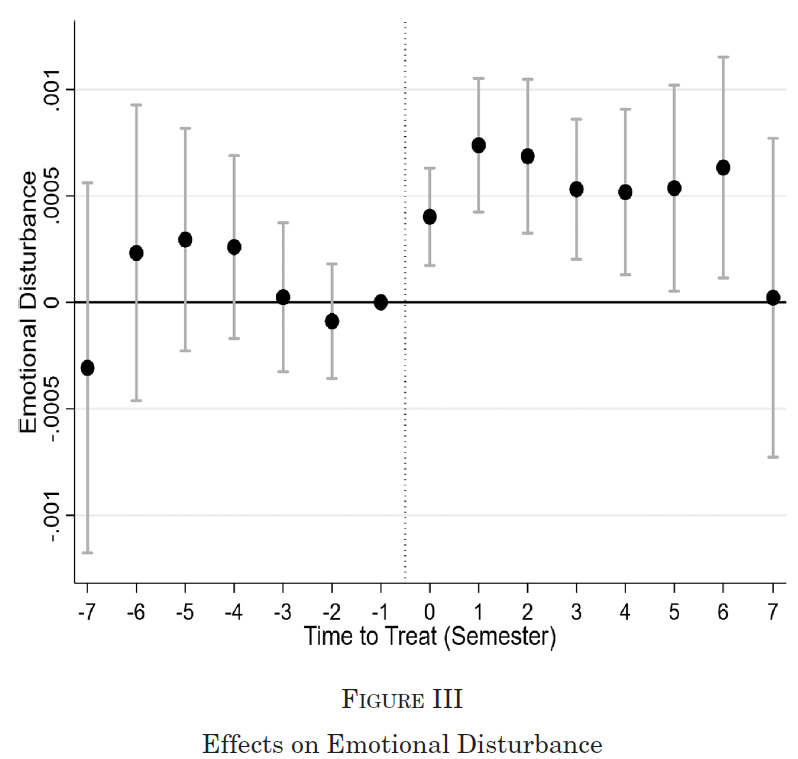
\includegraphics[scale = .55]{fig_tab/os20220113/F3}
  \end{figure}
\end{frame}

\begin{frame}{}
  \begin{itemize}
    \item little evidence of differential pretrends between treatment and control students (F-test of joint significance: $F = 1.15, p = .334$)
    \item Though the treatment estimates are small, ranging from 0.04 to 0.07 percentage points.
    \item Changes in emotional disturbance are also highly persistent after exposure.
    \begin{itemize}
      \item ED and psychological trauma are chronic conditions and often last for several years after the inciting incident (Famularo et al. 1996; Friedman et al. 1996)
      \item ED designations are sticky.
    \end{itemize}
  \end{itemize}
\end{frame}

\begin{frame}{Robustness}
  \begin{figure}
    \centering
    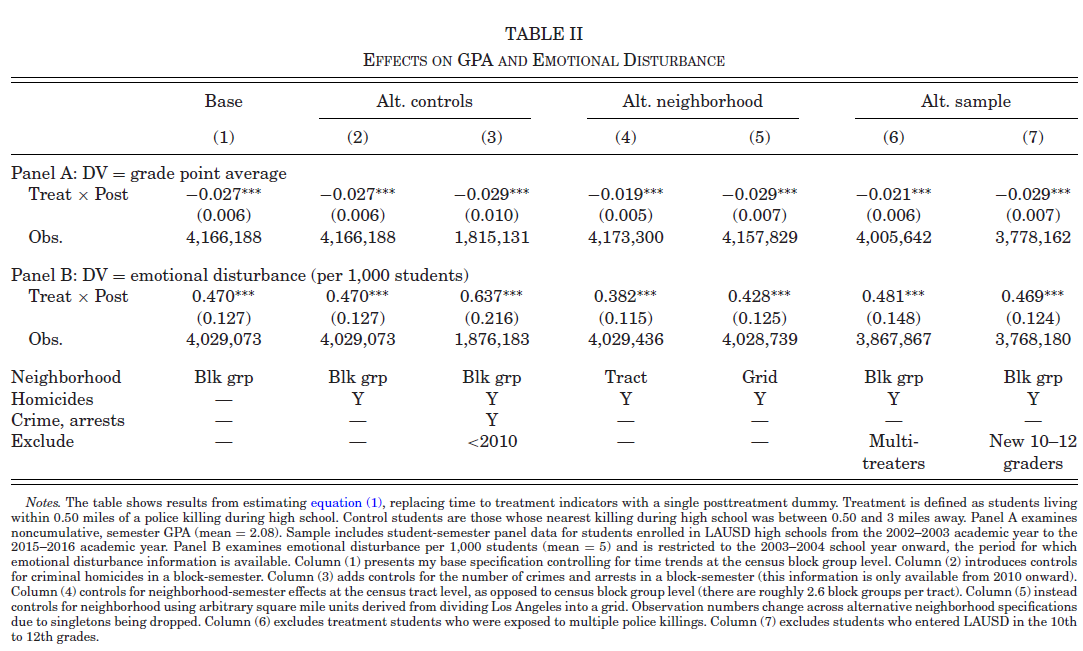
\includegraphics[scale = .55]{fig_tab/os20220113/T2}
  \end{figure}
\end{frame}

\begin{frame}{Additional Robustness Checks}
  \begin{figure}
    \centering
    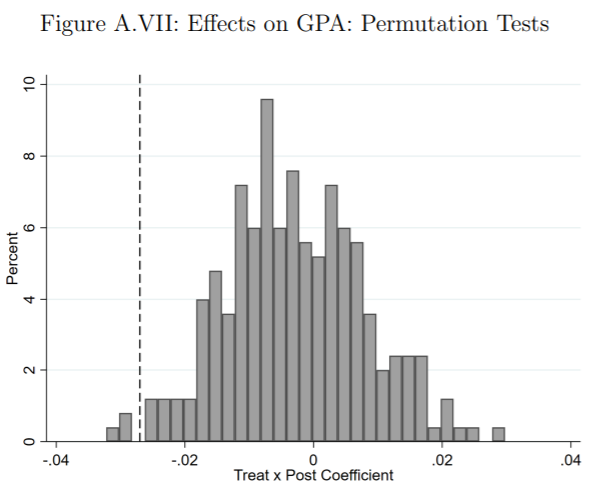
\includegraphics[scale = .4]{fig_tab/os20220113/FA7.png}
    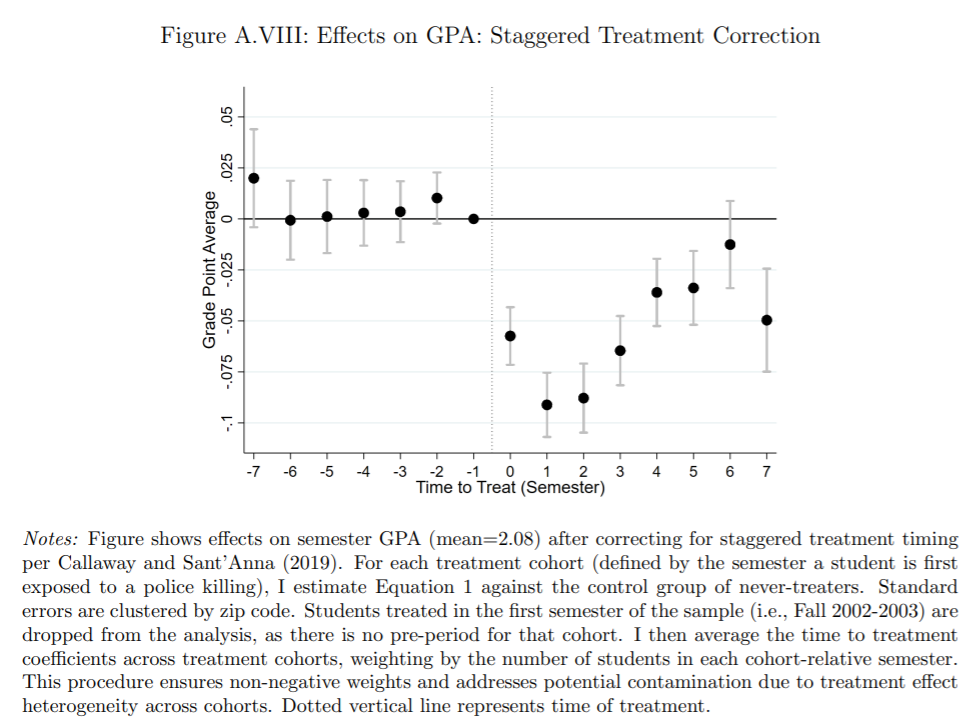
\includegraphics[scale = .4]{fig_tab/os20220113/FA8.png}
  \end{figure}
\end{frame}

\section{Mechanism}
\frame{\sectionpage}

\begin{frame}{Racial Differences}
  \begin{figure}
    \centering
    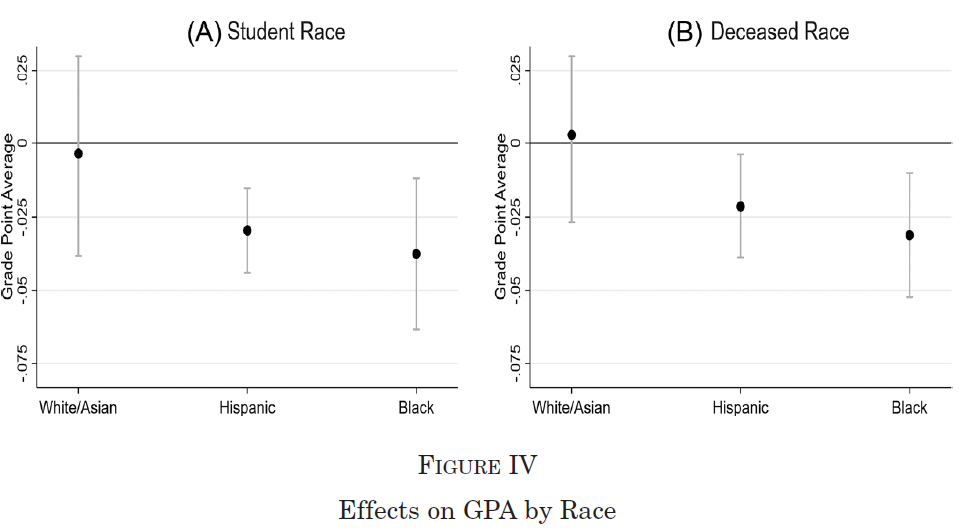
\includegraphics[scale = .55]{fig_tab/os20220113/F4}
  \end{figure}
\end{frame}

\begin{frame}{}
  \begin{itemize}
    \item Subsample analyses revealed that exposure to police killings has no impact on white and Asian students.
    \begin{itemize}
      \item Disproportionate burden police violence may have on underrepresented minorities (Gershenson and Hayes, 2018).
      \item Race is the single strongest predictor of perceptions of law enforcement (Taylor et al., 2001)
      \item blacks and Hispanics are significantly more likely to believe that police use of force is excessive or unjustified (Leiber, Nalla, and Farnworth 1998; Weitzer and Tuch 2002).
    \end{itemize}
  \end{itemize}
\end{frame}

\begin{frame}{the Deceased's Race}
  \begin{itemize}
    \item Because race is obviously not randomly  assigned, the effect heterogeneity of race of the deceased is likely to be correlated with other factors.
    \item flexible controls allowing for differential treatment effects along a range of neighborhood, incident, and individual characteristics.
    \begin{align*}
      y_{i, t} = & \delta_i + \lambda_{n, t} + \omega_{c, t} + \beta_{BH} \textit{Post} \times \textit{Shoot} \times \textit{BlackHispanic} \\
      &+ \beta_{WA} \textit{Post} \times \textit{Shoot} \times \textit{WhiteAsian} + \textit{Post} \times \textit{Shoot} \times \mathbf{X}_i \boldsymbol{\gamma} + \epsilon_{i, t}
    \end{align*}
    \begin{itemize}
      \item conditional on exposure, black and Hispanic students respond differently to police violence depending on the race of the person killed
    \end{itemize}
  \end{itemize}
\end{frame}

\begin{frame}{}
  \begin{figure}
    \centering
    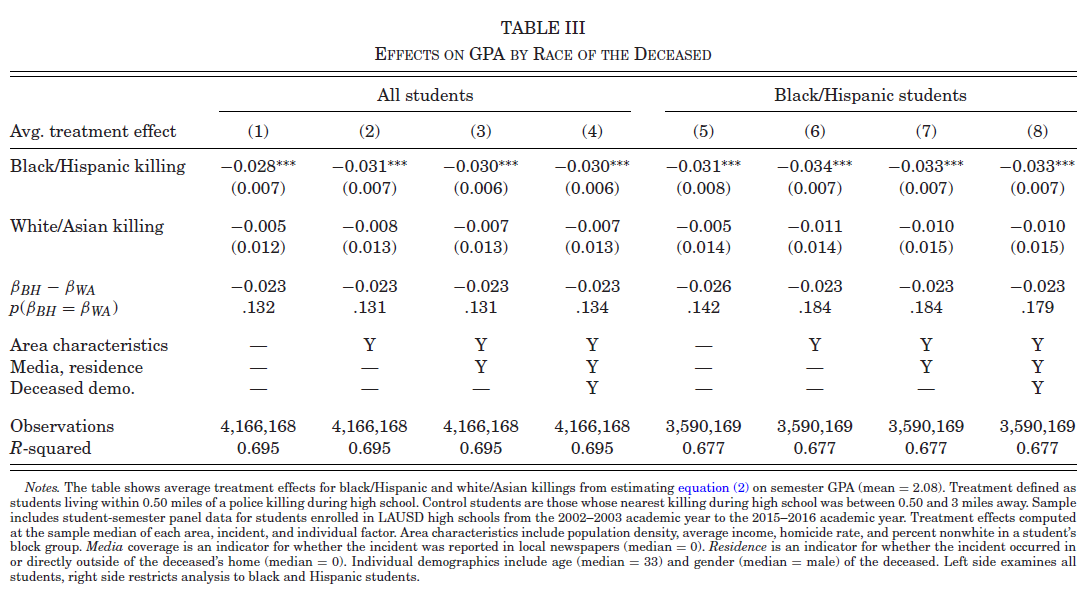
\includegraphics[scale = .55]{fig_tab/os20220113/T3}
  \end{figure}
\end{frame}

\begin{frame}{Weapon Type}
  \begin{figure}
    \centering
    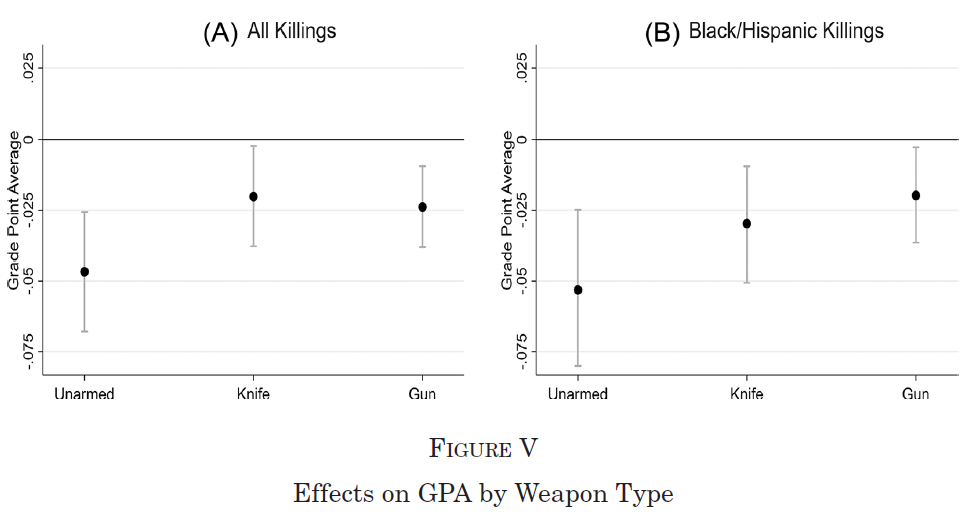
\includegraphics[scale = .55]{fig_tab/os20220113/F5}
  \end{figure}
\end{frame}

\begin{frame}{}
  \begin{itemize}
    \item The effects of police violence are unlikely to be driven by those incidents with the most gunfire or the deadliest shootouts.
    \item The most damaging events are police killings of unarmed individuals.
    \item the findings suggest that students may be responding to the perceived reasonableness or legitimacy of officer actions as much as to the use of force.
    \item However, community perceptions of “reasonableness” often depend on contextual factors similar to those assessed here, with police violence against unarmed minorities drawing particular concern (Hall, Hall, and Perry 2016)
  \end{itemize}
\end{frame}

\begin{frame}{Comparing Police and Criminal Violence}
  \begin{itemize}
    \item A simple model of violent exposure
    cannot fully explain the observed effects of police killings on student achievement.
    \begin{align*}
      y_{i, t} = & \delta_i + \lambda_{n, t} + \omega_{c, t} + \\
      & \sum_{\tau = -3}^3 \beta_{\tau} \textit{Police}_{\tau} + \sum_{\tau = -3}^3 \gamma_{\tau} \textit{NonPolice}_{\tau} + \mathbf{X}_{b, t} \boldsymbol{\gamma} + \epsilon_{i, t}
    \end{align*}
    \item The marginal effects differ suggests that students may view police killings and criminal homicides as unique phenomena and that different mechanisms might drive their to each.
    \begin{itemize}
      \item criminal homicides of whites/Asians and blacks/Hispanics are associated with nearly identical decreases in GPA.
    \end{itemize}
  \end{itemize}
\end{frame}

\begin{frame}{}
  \begin{figure}
    \centering
    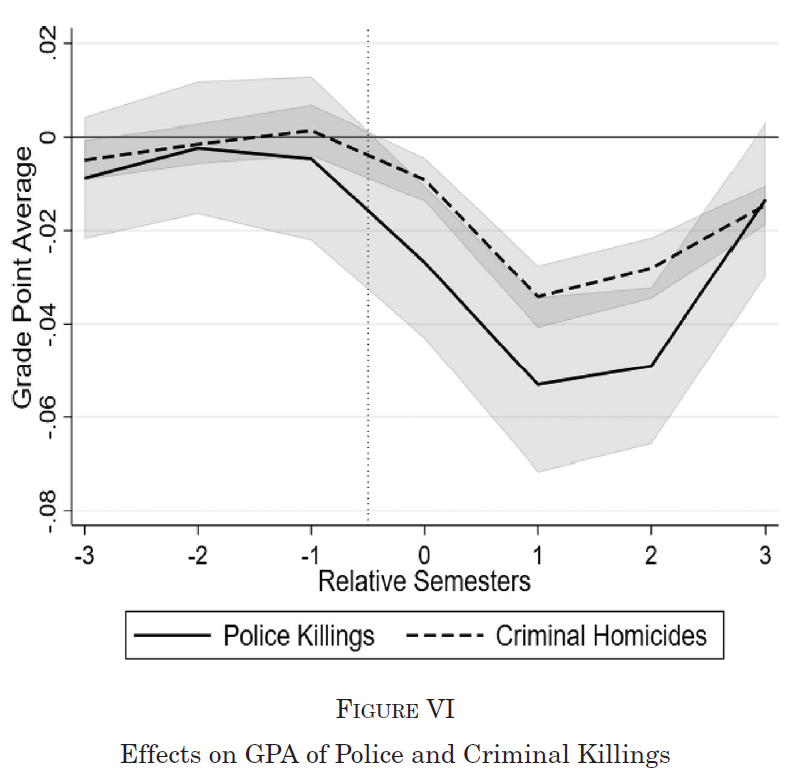
\includegraphics[scale = .55]{fig_tab/os20220113/F6}
  \end{figure}
\end{frame}

\section{Long-Run Effects}
\frame{\sectionpage}

\begin{frame}{Identification}
  \begin{itemize}
    \item Main regression equation cannot capture the long-run ramifications because exposure is absorbed by fixed effects.
    \begin{itemize}
      \item Compare graduation rates of students in expected grades.
    \end{itemize}
    \item For student $i$ of expected grade $g$,
    \begin{align*}
      y_{i, g} = \delta_{n, c} + \sum_{\tau = 9}^{16} \beta_{\tau} \textit{Shoot}_{i, g} \times \textit{Grade}_{\tau} + \lambda \textit{Shoot}_{i, g} + \mathbf{X}_i \boldsymbol{\gamma} + \epsilon_{i, g}
    \end{align*}
    \begin{itemize}
      \item Students with $\tau \geq 13$ are not exposed to the treatment.
      \item This specification does not allow to include indivudal fixed effects.
      \item demographic covariates: a student's school, race, sex, poverty status, household language, parental education, and eighth-grade proficiency
    \end{itemize}
  \end{itemize}
\end{frame}

\begin{frame}{Educational Attainment}
  \begin{figure}
    \centering
    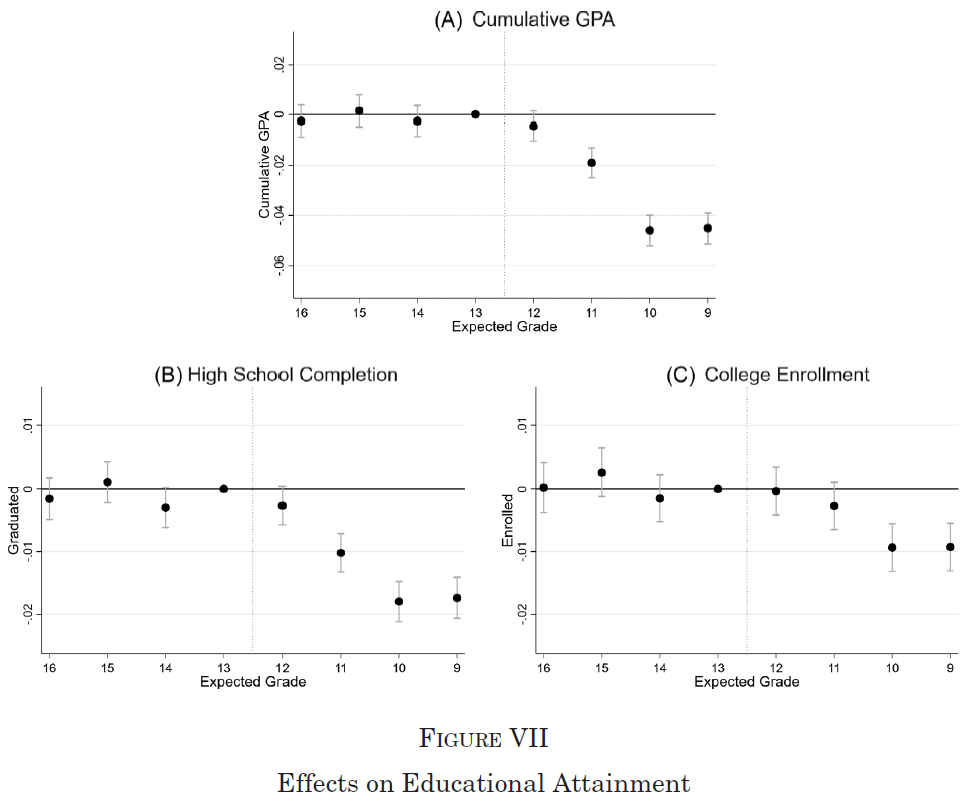
\includegraphics[scale = .5]{fig_tab/os20220113/F7}
  \end{figure}
\end{frame}

\begin{frame}{Educational Attaiment}
  \begin{itemize}
    \item Significant differences in long-run achievement associated with exposure to police violence.
    \begin{itemize}
      \item Average treatment estimate on cumulative GPA (0.029 points) $\fallingdotseq$ average estimate on semester GPA (0.027 points)
      \item Exposure in the 9th grade predicts a 1.7 percentage point decrease in the graduation rate.
      \item Exposure to police violence is associated with significant decreases in college enrollment among 9th and 10th graders of 0.09 percentage points
    \end{itemize}
  \end{itemize}
\end{frame}

\begin{frame}{Race-Specific Effects}
  \begin{figure}
    \centering
    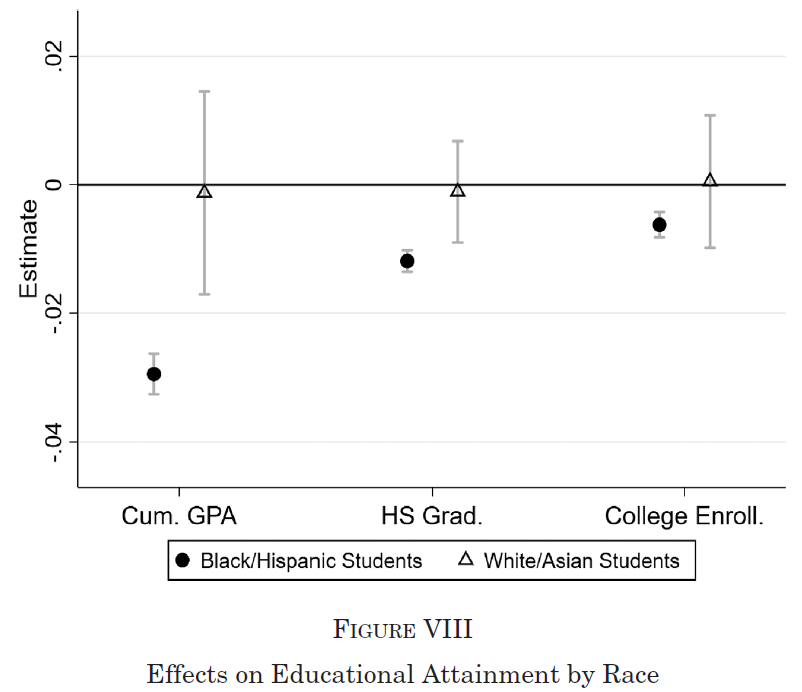
\includegraphics[scale = .55]{fig_tab/os20220113/F8}
  \end{figure}
\end{frame}

\begin{frame}{}
  \begin{itemize}
    \item The results indicate that police killings may have large long-run effects on local communities
    \begin{itemize}
      \item causal evidence supporting the link between adverse childhood experiences and educational attainment (Harris 1983; Broberg, Dyregrov, and Lilled 2005; Porche et al.
      2011)
    \end{itemize}
    \item However, police violence differs from many other forms of trauma in one important dimension.
  \end{itemize}
\end{frame}

\begin{frame}{Robustness}
  \begin{figure}
    \centering
    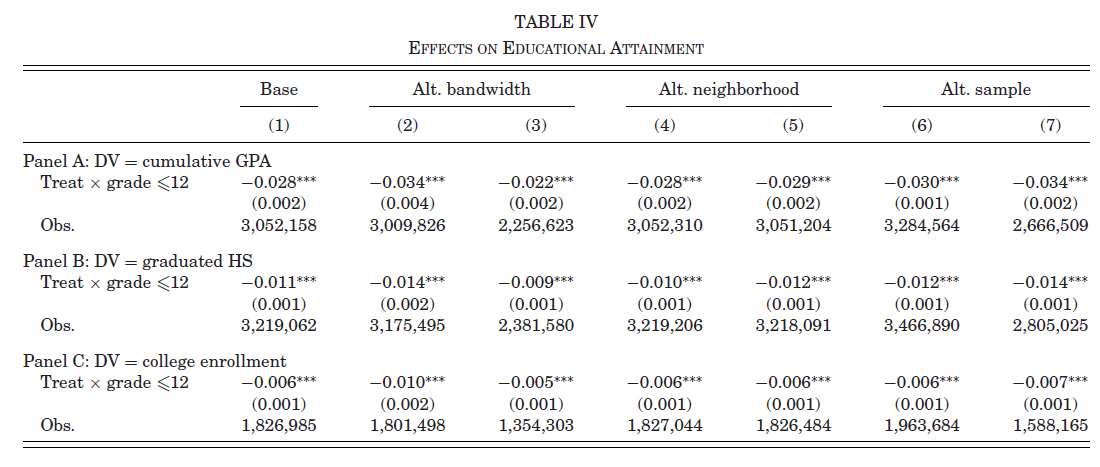
\includegraphics[scale = .4]{fig_tab/os20220113/T4}
    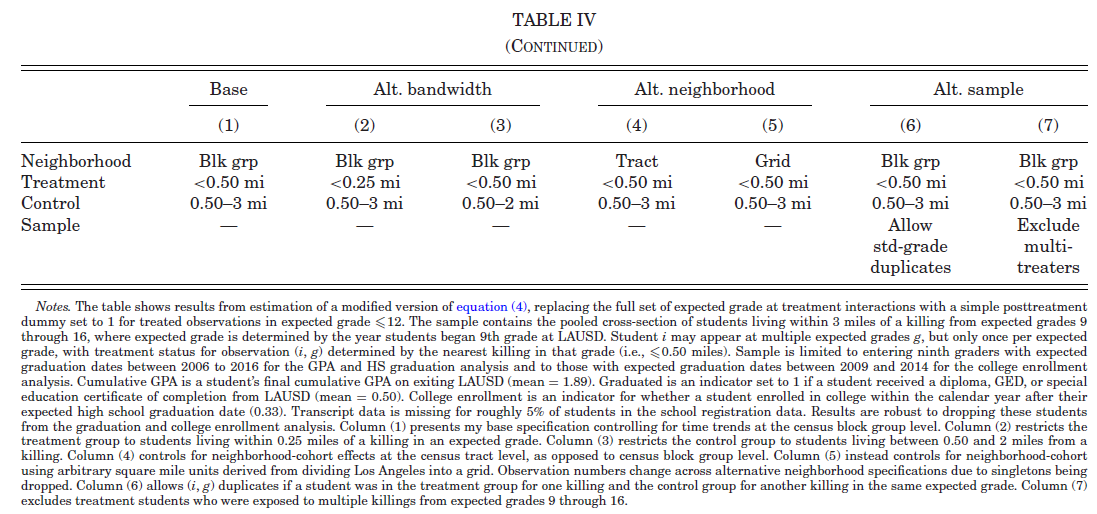
\includegraphics[scale = .4]{fig_tab/os20220113/T4_1}
  \end{figure}
\end{frame}

\section{Conclusion}
\frame{\sectionpage}
\begin{frame}{Concluding Remarks}
  \begin{itemize}
    \item This article provides the first causal evidence of the impact of police killings on nearby students.
    \item Results indicate that police violence may
    exacerbate racial inequality in education
    \item This paper does not account for effects on younger children or for other returns to schooling (Lochner and Moretti 2004), this figure likely underestimates the total educational costs of police killings
    \item Critically examine the appropriate role of law enforcement in local
    communities.
  \end{itemize}
\end{frame}

\end{document}
